% -*- coding: utf-8 -*-
%-------------------------designed by zcf--------------
\documentclass[UTF8,a4paper,10pt]{ctexart}
\usepackage[left=3.17cm, right=3.17cm, top=2.74cm, bottom=2.74cm]{geometry}
\usepackage{amsmath}
\usepackage{graphicx,subfig}
\usepackage{float}
\usepackage{cite}
\usepackage{caption}
\usepackage{enumerate}
\usepackage{booktabs} %表格
\usepackage{multirow}
\newcommand{\tabincell}[2]{\begin{tabular}{@{}#1@{}}#2\end{tabular}}  %表格强制换行
%-------------------------字体设置--------------
\usepackage{times} 
\newcommand{\yihao}{\fontsize{26pt}{36pt}\selectfont}           % 一号, 1.4 倍行距
\newcommand{\erhao}{\fontsize{22pt}{28pt}\selectfont}          % 二号, 1.25倍行距
\newcommand{\xiaoer}{\fontsize{18pt}{18pt}\selectfont}          % 小二, 单倍行距
\newcommand{\sanhao}{\fontsize{16pt}{24pt}\selectfont}  %三号字
\newcommand{\xiaosan}{\fontsize{15pt}{22pt}\selectfont}        % 小三, 1.5倍行距
\newcommand{\sihao}{\fontsize{14pt}{21pt}\selectfont}            % 四号, 1.5 倍行距
\newcommand{\banxiaosi}{\fontsize{13pt}{19.5pt}\selectfont}    % 半小四, 1.5倍行距
\newcommand{\xiaosi}{\fontsize{12pt}{18pt}\selectfont}            % 小四, 1.5倍行距
\newcommand{\dawuhao}{\fontsize{11pt}{11pt}\selectfont}       % 大五号, 单倍行距
\newcommand{\wuhao}{\fontsize{10.5pt}{15.75pt}\selectfont}    % 五号, 单倍行距
%-------------------------章节名----------------
\usepackage{ctexcap} 
\CTEXsetup[name={,、},number={ \chinese{section}}]{section}
\CTEXsetup[name={(,)},number={\chinese{subsection}}]{subsection}
\CTEXsetup[name={,.},number={\arabic{subsubsection}}]{subsubsection}
%-------------------------页眉页脚--------------
\usepackage{fancyhdr}
\pagestyle{fancy}
\lhead{\kaishu \leftmark}
% \chead{}
\rhead{\kaishu 计算机系统设计实验报告}%加粗\bfseries 
\lfoot{}
\cfoot{\thepage}
\rfoot{}
\renewcommand{\headrulewidth}{0.1pt}  
\renewcommand{\footrulewidth}{0pt}%去掉横线
\newcommand{\HRule}{\rule{\linewidth}{0.5mm}}%标题横线
\newcommand{\HRulegrossa}{\rule{\linewidth}{1.2mm}}
%-----------------------伪代码------------------
\usepackage{algorithm}  
\usepackage{algorithmicx}  
\usepackage{algpseudocode}  
\floatname{algorithm}{Algorithm}  
\renewcommand{\algorithmicrequire}{\textbf{Input:}}  
\renewcommand{\algorithmicensure}{\textbf{Output:}} 
\usepackage{lipsum}  
\makeatletter
\newenvironment{breakablealgorithm}
  {% \begin{breakablealgorithm}
  \begin{center}
     \refstepcounter{algorithm}% New algorithm
     \hrule height.8pt depth0pt \kern2pt% \@fs@pre for \@fs@ruled
     \renewcommand{\caption}[2][\relax]{% Make a new \caption
      {\raggedright\textbf{\ALG@name~\thealgorithm} ##2\par}%
      \ifx\relax##1\relax % #1 is \relax
         \addcontentsline{loa}{algorithm}{\protect\numberline{\thealgorithm}##2}%
      \else % #1 is not \relax
         \addcontentsline{loa}{algorithm}{\protect\numberline{\thealgorithm}##1}%
      \fi
      \kern2pt\hrule\kern2pt
     }
  }{% \end{breakablealgorithm}
     \kern2pt\hrule\relax% \@fs@post for \@fs@ruled
  \end{center}
  }
\makeatother
%------------------------代码-------------------
\usepackage{xcolor} 
\usepackage{listings} 
\usepackage{fontspec}
\newfontfamily\menlo{Menlo}
\setmonofont[Mapping={}]{Monaco} 
\definecolor{mygreen}{rgb}{0,0.6,0}
\definecolor{mygray}{rgb}{0.5,0.5,0.5}
\definecolor{mymauve}{rgb}{0.58,0,0.82}
\lstset{ %
backgroundcolor=\color{white},   % choose the background color
basicstyle=\footnotesize\ttfamily,        % size of fonts used for the code
columns=fullflexible,
breaklines=true,                 % automatic line breaking only at whitespace
captionpos=b,                    % sets the caption-position to bottom
tabsize=4,
commentstyle=\color{mygreen},    % comment style
escapeinside={\%*}{*)},          % if you want to add LaTeX within your code
keywordstyle=\color{blue},       % keyword style
stringstyle=\color{mymauve}\ttfamily,     % string literal style
frame=single,
rulesepcolor=\color{red!20!green!20!blue!20},
numbers=left,
 numberstyle=\tiny\menlo
% identifierstyle=\color{red},
% language=c++,
}
%------------超链接----------
\usepackage[colorlinks,linkcolor=black,anchorcolor=blue]{hyperref}
%------------------------TODO-------------------
\usepackage{enumitem,amssymb}
\newlist{todolist}{itemize}{2}
\setlist[todolist]{label=$\square$}
% for check symbol 
\usepackage{pifont}
\newcommand{\cmark}{\ding{51}}%
\newcommand{\xmark}{\ding{55}}%
\newcommand{\done}{\rlap{$\square$}{\raisebox{2pt}{\large\hspace{1pt}\cmark}}\hspace{-2.5pt}}
\newcommand{\wontfix}{\rlap{$\square$}{\large\hspace{1pt}\xmark}}
%------------------------水印-------------------
\usepackage{tikz}
\usepackage{xcolor}
\usepackage{eso-pic}

\newcommand{\watermark}[3]{\AddToShipoutPictureBG{
\parbox[b][\paperheight]{\paperwidth}{
\vfill%
\centering%
\tikz[remember picture, overlay]%
  \node [rotate = #1, scale = #2] at (current page.center)%
    {\textcolor{gray!80!cyan!30!magenta!30}{#3}};
\vfill}}}



%———————————————————————————————————————————正文———————————————————————————————————————————————
%----------------------------------------------
\begin{document}
\begin{titlepage}
    \begin{center}
    
\includegraphics[width=0.8\textwidth]{NKU.png}\\[1cm]    
    \textsc{\Huge \kaishu{\textbf{南\ \ \ \ \ \ 开\ \ \ \ \ \ 大\ \ \ \ \ \ 学}} }\\[0.9cm]
    \textsc{\huge \kaishu{\textbf{计\ \ 算\ \ 机\ \ 学\ \ 院}}}\\[0.5cm]
    \textsc{\Large \textbf{计算机系统设计实验报告}}\\[0.8cm]
    \HRule \\[0.9cm]
    { \LARGE \bfseries PA3实验报告}\\[0.4cm]
    \HRule \\[2.0cm]
    \centering
    \textsc{\LARGE \kaishu{朱浩泽\ 1911530}}\\[0.5cm]
    \textsc{\LARGE \kaishu{年级\ :\ 2019级}}\\[0.5cm]
    \textsc{\LARGE \kaishu{专业\ :\ 计算机科学与技术}}\\[0.5cm]
    \textsc{\LARGE \kaishu{指导教师\ :\ 卢冶}}\\[0.5cm]
    \vfill
    {\Large \today}
    \end{center}
\end{titlepage}
% -------------摘------要--------------
\newpage
% \thispagestyle{empty}
% \renewcommand{\abstractname}{\kaishu \sihao \textbf{摘要}}
%     \begin{abstract}

%         \noindent  %顶格
%         \textbf{\\\ 关键字:Parallel}\textbf{} \\\ \\\
%     \end{abstract}
% ----------------------------------------------------------------
\tableofcontents
% ----------------------------------------------------------------
\newpage
\watermark{60}{10}{NKU}
\setcounter{page}{1}
\section{概述}
\subsection{实验目的}
\begin{enumerate}
  \item 了解基础设施测试、调试的基本框架与思想
  \item 实现I/O设备的基本操作
  \item 掌握高级语言程序中的各种类型变量对应的表示形式
  \item 学习指令周期与指令执行过程,并简单实现现代指令系统
  \item 了解冯诺依曼计算机体系结构
  \item 在高级语言程序中的变量、机器数和底层硬件(寄存器、加法器、ALU等)之间建立关联
\end{enumerate}

\subsection{实验内容}
\begin{enumerate}
  \item 实现基本的指令
  \item 运行第一个 C 程序
  \item 补全更多的指令并进行diff-text
  \begin{enumerate}
    \item 完善nemu/src/cpu/exec/exec.c中的opcode\_table
    \item 完善nemu/include/cpu/rtl.h中的基本操作函数
    \item 完善nemu/src/cpu/* 中的执行函数。(执行函数统一通过宏make\_EHelper 定义)
  \end{enumerate}
  \item 学习I/O的原理,实现屏幕的打印和键盘的输入
\end{enumerate}

\section{阶段一}
\subsection{环境配置}
首先,我们要配置好环境变量,由于我在虚拟机终端中使用的是zsh(为了使用oh-my-zsh),所以我们要在zsh的配置中(Home/Username/.zshrc)添加如下内容:
\begin{lstlisting}[]
export NEMU_HOME=~/PA/ics2017/nemu
export AM_HOME=~/PA/ics2017/nexus-am
export NAVY_HOME=~/PA/ics2017/navy-apps
\end{lstlisting}



\subsection{寄存器传输语言}
在程序执行执行过程中,我们都是使用RTL(寄存器传输语言)来实现该过程。首先,需要在 nemu/include/cpu/reg.h 文件中补充EFlags的标志位
\begin{lstlisting}[language=C]
  struct bs {
    unsigned int CF:1;

    unsigned int one:1;
    unsigned int :4;
    unsigned int ZF:1;
    unsigned int SF:1;

    unsigned int :1;
    unsigned int IF:1;
    unsigned int :1;
    unsigned int OF:1;
    unsigned int :20;
  } eflags;
\end{lstlisting}

这些Eflags将在nemu/src/monitor/monitor.c中进行初始化, 并在nemu/src/cpu/arith.c中进行标志位的设置进行减法计算
\begin{lstlisting}[language = C]
static inline void restart() {
  /* Set the initial instruction pointer. */
  cpu.eip = ENTRY_START;

  unsigned int origin = 2;
  memcpy(&cpu.eflags, &origin, sizeof(cpu.eflags));

#ifdef DIFF_TEST
  init_qemu_reg();
#endif
}
\end{lstlisting}
\begin{lstlisting}[language = C]
static inline void eflags_modify() {
  rtl_sub(&t2, &id_dest -> val, &id_src -> val);
  rtl_update_ZFSF(&t2, id_dest -> width);
  rtl_sltu(&t0, &id_dest -> val, &id_src -> val);
  rtl_set_CF(&t0);
  rtl_xor(&t0, &id_dest->val, &id_src->val);
  rtl_xor(&t1, &id_dest->val, &t2);
  rtl_and(&t0, &t0, &t1);
  rtl_msb(&t0, &t0, id_dest->width);
  rtl_set_OF(&t0);
}
\end{lstlisting}

rtl指令在nemu/include/cpu/rtl.h文件中。在rtl.h中,指令分为两部分,一部分是rtl指令,另一部分则是rtl伪指令, 它们是通过rtl指令实现的。

我们实现rtl\_push函数让其修改栈顶,并将指针src1中的内容写入栈。
\begin{lstlisting}[language = C++]
static inline void rtl_push(const rtlreg_t* src1) {
  // esp <- esp - 4
  // M[esp] <- src1
  //TODO();
  rtl_subi(&cpu.esp, &cpu.esp, 4);
  rtl_sm(&cpu.esp, 4, src1);
}
\end{lstlisting}

我们实现rtl\_pop函数让其将rtl\_pop读取的数据写入到通用寄存器中。
\begin{lstlisting}[language = C++]
static inline void rtl_pop(rtlreg_t* dest) {
    // dest <- M[esp]
    rtl_lm(dest,&cpu.esp,4);
    // esp <- esp + 4
    rtl_addi(&cpu.esp,&cpu.esp,4);
  }
\end{lstlisting}

 与此同时,我们还实现了其他指令的编写,如下:

EFLAGS 寄存器的标志位读写函数
\begin{lstlisting}[language = C]
#define make_rtl_arith_logic(name) \
static inline void concat(rtl_, name) (rtlreg_t* dest, const rtlreg_t* src1, const rtlreg_t* src2) { \
  *dest = concat(c_, name) (*src1, *src2); \
} \
static inline void concat3(rtl_, name, i) (rtlreg_t* dest, const rtlreg_t* src1, int imm) { \
  *dest = concat(c_, name) (*src1, imm); \
}
\end{lstlisting}

EFLAGS 寄存器的标志位更新函数
\begin{lstlisting}[language = C]
static inline void rtl_eq0(rtlreg_t* dest, const rtlreg_t* src1) {
  rtl_sltui(dest, src1, 1);
}

static inline void rtl_eqi(rtlreg_t* dest, const rtlreg_t* src1, int imm) {
  rtl_xori(dest, src1, imm);
  rtl_eq0(dest, dest);
}

static inline void rtl_neq0(rtlreg_t* dest, const rtlreg_t* src1) {
  rtl_eq0(dest, src1);
  rtl_eq0(dest, dest);
}

static inline void rtl_msb(rtlreg_t* dest, const rtlreg_t* src1, int width) {
  rtl_shri(dest, src1, width*8-1);
  rtl_andi(dest, dest, 0x1);
}

static inline void rtl_update_ZF(const rtlreg_t* result, int width) {
  rtl_andi(&t0, result, (0xffffffffu >> (4-width)*8));
  rtl_eq0(&t0, &t0);
  rtl_set_ZF(&t0);
}

static inline void rtl_update_SF(const rtlreg_t* result, int width) {
  assert(result != &t0);
  rtl_msb(&t0, result, width);
  rtl_set_SF(&t0);
}
\end{lstlisting}

实现立即数加法
\begin{lstlisting}[language = C]
static inline void rtl_mv(rtlreg_t* dest, const rtlreg_t *src1) {
  rtl_addi(dest, src1, 0);
}
\end{lstlisting}

实现逻辑非运算
\begin{lstlisting}[language = C]
static inline void rtl_not(rtlreg_t* dest) {
  rtl_xori(dest, dest, 0xffffffff);
}
\end{lstlisting}

符号拓展,主要与最高位有关
\begin{lstlisting}[language = C]
static inline void rtl_sext(rtlreg_t* dest, const rtlreg_t* src1, int width) {
  if(width == 0) {
    rtl_mv(dest, src1);
  }
  else {
    rtl_shli(dest, src1, (4 - width) * 8);
    rtl_sari(dest, dest, (4 - width) * 8);
  }
}
\end{lstlisting}

\subsection{尝试运行dummy.c}
首先我们什么都不做,运行 make ARCH=x86-nemu ALL=dummy,一定是报错。我们通过查看反汇编的代码,可以看出是call指令和endbr指令没有实现。我们通过这种方法进行逐一操作,对指令进行补充。
\begin{center}
  \includegraphics*[scale = 0.3]{1.png}
\end{center}

在这一阶段,我们需要实现的指令有如下
\begin{table}[!htbp]
  \centering
  \begin{tabular}{ccccccccccc}
  \toprule  
  指令& 编码\\
  \midrule
  call& e8\\
  push& 50\\
  sub&  83\\
  \bottomrule
  \end{tabular}
  \begin{tabular}{ccccccccccc}
    \toprule  
    指令& 编码\\
    \midrule
    xor& 31\\
    pop& 58\\
    ret& c3\\
    \bottomrule
    \end{tabular}
\end{table}

可以看出,每个指令都有自己的编号,这是通过查阅i386的指令手册来得到的,其第一个16进制数的是指令的opcode。
\begin{center}
  \includegraphics*[scale = 0.35]{2.png}
\end{center}

每条指令分别需要执行函数和译码函数,译码函数的主要作用是从opcode的后三位中读取通用寄存器的编号,过程是读取 decoding.opcode 中标志的寄存器, 将寄存器的内容放入 op->val 中。nemu/src/cpu/exec/exec.c中的opcode\_table的每一条记录包括译码函数、执行函数、(两个)操作数的宽度,如下
\begin{lstlisting}[language = C]
typedef struct {
  DHelper decode;
  EHelper execute;
  int width;
} opcode_entry;
\end{lstlisting}

我们将在这些指令的编号填写在opcode\_table中,如下
\begin{lstlisting}[language = C]
  /* 0x50 */  IDEX(r,push), IDEX(r,push), IDEX(r,push), IDEX(r,push),
  /* 0x54 */  IDEX(r,push), IDEX(r,push), IDEX(r,push), IDEX(r,push),
  //...
  //call
  /* 0xe8 */  IDEX(J,call), IDEX(J,jmp), EMPTY, IDEXW(J,jmp,1),
  ……
\end{lstlisting}

然后在nemu/src/cpu/exec/all-instr.h补全执行函数,如下(一次性全部展示,后续将不再说明)
\begin{lstlisting}[language = C++]
make_EHelper(mov);

make_EHelper(operand_size);

make_EHelper(inv);
make_EHelper(nemu_trap);
make_EHelper(call);
make_EHelper(call_rm);
make_EHelper(push);
make_EHelper(pop);
make_EHelper(sub);
make_EHelper(xor);
make_EHelper(ret);

make_EHelper(endbr);

make_EHelper(add);
make_EHelper(inc);
make_EHelper(dec);
make_EHelper(cmp);
make_EHelper(neg);
make_EHelper(adc);
make_EHelper(sbb);
make_EHelper(mul);
make_EHelper(imul1);
make_EHelper(imul2);
make_EHelper(imul3);
make_EHelper(div);
make_EHelper(idiv);

make_EHelper(not);
make_EHelper(and);
make_EHelper(or);
make_EHelper(xor);
make_EHelper(sal);
make_EHelper(shl);
make_EHelper(shr);
make_EHelper(sar);
make_EHelper(rol);
make_EHelper(setcc);
make_EHelper(test);

make_EHelper(leave);
make_EHelper(cltd);
make_EHelper(cwtl);
make_EHelper(movsx);
make_EHelper(movzx);

make_EHelper(jmp);
make_EHelper(jmp_rm);
make_EHelper(jcc);

make_EHelper(lea);
make_EHelper(nop);

make_EHelper(in);
make_EHelper(out);

make_EHelper(lidt);
make_EHelper(int);

make_EHelper(pusha);
make_EHelper(popa);
make_EHelper(iret);

make_EHelper(mov_store_cr);
\end{lstlisting}

在补充完函数定义后nemu/src/cpu/exec中的执行函数和nemu/src/cpu/exec/decode.c中的译码函数进行编写
\begin{itemize}
  \item push
  
  调用上一节中所写的rtl\_push执行函数进行写栈,代码如下
  \begin{lstlisting}[language = C]
  make_EHelper(push) {
    //TODO();
    rtl_push(&id_dest -> val);
    print_asm_template1(push); 
  }
  \end{lstlisting}
  \item pop
  
  调用上一节中所写的rtl\_pop执行函数进行读栈,将读取的数据写入到通用寄存器中,代码如下
  \begin{lstlisting}[language = C]
make_EHelper(pop) {
  // TODO();
  rtl_pop(&t2);
  operand_write(id_dest, &t2);
  print_asm_template1(pop);
}
\end{lstlisting}
  
\item call
    
为J形指令,操作数仅一个立即数。CPU 的跳转目标地址=当前 eip+立即数 offset。所以我们编写nemu/src/cpu/decode/decode.c中的译码函数make\_DHelper(J),调用decode\_op\_SI 函数实现立即数的读取,并更新jmp\_eip。
\begin{lstlisting}[language = C]
make_DHelper(J) {
  decode_op_SI(eip, id_dest, false);
  // the target address can be computed in the decode stage
  decoding.jmp_eip = id_dest->simm + *eip;
}  
\end{lstlisting}
然后我们编写nemu/src/cpu/exe/control.c中的执行函数make\_EHelper(call)
\begin{lstlisting}[language = C]
make_EHelper(call) {
  // the target address is calculated at the decode stage
  //TODO();
  rtl_li(&t2, decoding.seq_eip);
  rtl_push(&t2);

  decoding.is_jmp = 1;

  print_asm("call %x", decoding.jmp_eip);
}
\end{lstlisting}
  \item sub
  
  编写译码函数make\_DHelper(I2a),调用 decode\_op\_a读取 AX/EAX中的数据写入 id\_dest,调用 decode\_op\_I 读取立即数并存入 id\_src
  \begin{lstlisting}[language = C]
make_DHelper(I2a) {
  decode_op_a(eip, id_dest, true);
  decode_op_I(eip, id_src, true);
}
\end{lstlisting}
  编写执行函数make\_EHelper(sub),调用 eflags\_modify()计算减法并将值写回寄存器
  \begin{lstlisting}[language = C]
make_EHelper(sub) {
  // TODO();

  eflags_modify();
  operand_write(id_dest, &t2);
  print_asm_template2(sub);
}
\end{lstlisting}

  \item xor
  
  实现执行函数make\_Ehelper(xor)
  \begin{lstlisting}[language = C]
make_EHelper(xor) {
  // TODO();
  rtl_xor(&t2, &id_dest -> val, &id_src -> val);
  operand_write(id_dest, &t2);

  rtl_update_ZFSF(&t2, id_dest -> width);

  rtl_set_CF(&tzero);
  rtl_set_OF(&tzero);

  print_asm_template2(xor);
}
\end{lstlisting}

  \item ret
  
  实现执行函数make\_EHelper(ret),用栈的数据修改IP的内容,实现近转移
  \begin{lstlisting}[language = C]
make_EHelper(ret) {
  // TODO();
  rtl_pop(&t2);
  decoding.jmp_eip = t2;
  decoding.is_jmp = 1;
  print_asm("ret");
}
\end{lstlisting}

在补充完这些所需要的指令后,我们再次执行 make ARCH=x86-nemu ALL=dummy,可以看到这时dummy.c可以在我们的nemu中正确的运行。
\begin{center}
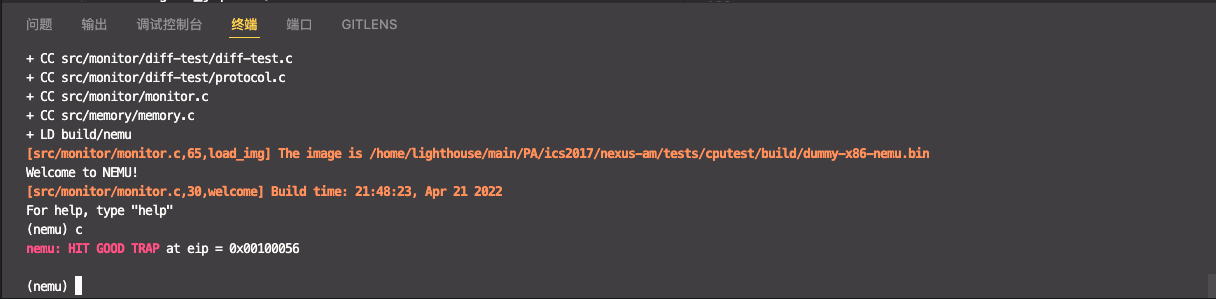
\includegraphics[width=0.9\textwidth]{dummy.png}
\end{center}
\end{itemize}

我们可以看出,指令执行的大概过程是在exec.c中,我们通过exec\_wrapper()函数开始执行指令,将当前的eip放进译码信息中(主要是为了诸如jmp,call等转移指令),之后执行exec\_real()函数。在该函数中,我们首先从当前地址中取出一个字节。在指令集执行过程中,我们都是先取 出一个字节的操作码,从opcode\_table中寻找匹配项,再执行对应的译码程序和执行程序,完成程序指令的执行。

\section{阶段二}

\section{感想与体会}
opcode有一位的和两位的


















































% \section{概述}
% %——————————————————————————————————————
% \subsection{第一节}
% 如图\ref{fig:1}所示
% \begin{figure}[H]
%     \centering
%     
\includegraphics[scale=0.3]{NKU.png}
%     \caption{Caption}
%     \label{fig:1}
% \end{figure}

% 表
% \begin{table}[!htbp]
%   \centering
%   \begin{tabular}{ccccccccccc}
%   \toprule  
%   N/n$\backslash$Algo& naive-conv& naive-pool& omp-conv& omp-pool\\
%   \midrule
%   64/2& 0.0167& 0.01255& 0.04142& 0.03799\\
%   64/4& 0.03599&0.0394& 0.0458& 0.0421\\
%   \bottomrule
%   \end{tabular}
%   \caption{性能测试结果(4线程)(单位:ms)}
% \end{table}

% 带单元格表格
% \begin{table}[!htbp]
%   \centering
%   \begin{tabular}{|c|c|c|c|c|c|c|}
%   \hline
%   \multicolumn{2}{|c|}{ \multirow{2}*{$Cost$} }& \multicolumn{5}{c|}{To}\\
%   \cline{3-7}
%   \multicolumn{2}{|c|}{}&$A$&$B$&$C$&$D$&$E$\\
%   \hline
%   \multirow{3}*{From}&$B$&7&0&1&3&8\\
%   \cline{2-7}
%   &$C$&8&1&0&2&7\\
%   \cline{2-7}
%   &$D$&8&3&2&0&5\\
%   \hline
%   \end{tabular}
%   \caption{结点C距离向量表(无毒性逆转)}
% \end{table}

% %——————————————————————————————————————
% \subsection{第二节}
% 伪代码

% \begin{breakablealgorithm} 
%   \caption{初始化obj文件信息——对应MeshSimplify类中readfile函数,Face类calMatrix函数} 
%   \begin{algorithmic}[1] %每行显示行号  
%       \Require obj文件,顶点、边、面列表
%       \Ensure 是否读取成功
%       \Function {calMatrix}{$Face$}  
%               \State $normal \gets e1×e2$  
%               \State $normal \gets normal/normal.length$
%               \State $temp[] \gets {normal.x, normal.y, normal.z, normal· Face.v1}$
%               \State $Matrix[i][j]=temp[i] * temp[j]$ 
%               \State \Return{$Matrix$}  
%       \EndFunction
%       \State 根据obj的v和f区分点面信息,读取并加入列表
%       \State $scale \gets $记录点坐标中距离原点最远的分量,以便后续OpenGL进行显示
%       \State $ori \gets $记录中心点,便于OpenGL显示在中心位置,避免有的obj偏移原点较多
%       \State 根据三角面片信息,计算一个面的三条边
%       \State 计算每个面的矩阵$\gets calMatrix$
%       \State 将每个面的矩阵加到各点,由点维护\\
%       \Return True
%   \end{algorithmic}  
% \end{breakablealgorithm}

% 代码
% \begin{lstlisting}[title=逐列访问平凡算法,frame=trbl,language={C++}]
%   void ord()   
%   {
%       double head,tail,freq,head1,tail1,timess=0; // timers
%       init(N);
%       QueryPerformanceFrequency((LARGE_INTEGER *)&freq );
%       QueryPerformanceCounter((LARGE_INTEGER *)&head);
%       for (int i=0; i<NN; i++)
%           for (int j=0; j<NN; j++)
%               col_sum[i] += (b[j][i]*a[j]);
%       QueryPerformanceCounter ((LARGE_INTEGER *)& tail) ;
%       cout << "\nordCol" <<(tail-head)*1000.0 / freq<< "ms" << endl;
%   }
% \end{lstlisting}


% %——————————————————————————————————————
% \subsection{第三节}

% 参考文献\cite{adams1995hitchhiker}\cite{shin2016deep}
    
% 多行公式
% \begin{align}
%   a+b = a + b \\
%   \frac{a+b}{a-b}
% \end{align}

% 行内公式:$\sum^N_{i=1}$

% \textbf{超链接}  \href{http://youtube.com/}{YouTube}

% 带标号枚举
% \begin{enumerate}
%   \item 1
%   \item 2
% \end{enumerate}

% 不带标号枚举
% \begin{itemize}
%   \item 1
%   \item 2
% \end{itemize}

% \xiaosi{切换字体大小}

% %----------------------------------------------------------------
% \section{总结}

% %----------------------------------------------------------------
% \newpage
% \bibliographystyle{plain}
% \bibliography{references} 
\end{document}
